%%
%% Author: dariochinelli
%% 2020-10-13
%%

\section{Meccanica Statistica}

Considero un sistema di $N$ particelle e suppongo che ognuna di queste si trovi in un certo stato dell'energia.
Assumo che tali stati siano discreti.

$$ N = n_1 + n_2 + n_3 + ... = \sum_s n_s \Rightarrow U_{tot} = n_1 E_1 + n_2 E_2 + ... = \sum_s n_s E_s $$

Dove $n_s$ è il numero di particelle nello stato $s$.
Assumiamo che queste particelle non interagiscano tra loro, allora posso attribuire ad ogni particella un potenziale che dipende solo dalle coordinate:
$N$ è costante e, se il sistema è isolato, anche $U_{tot}$ è costante.

$$ E_i = E_k + E_{pot} $$

Esistono più distribuzioni possibili per le particelle fra i vari livelli energetici, che sono dette \underline{partizioni}.

Si assume che per ogni stato macroscopico del sistema ci sia una partizione più probabile delle altre, nella quale si ha equilibrio statico,
situazione che permane se il sistema è isolato.
Vediamo tre modelli statistici.


\begin{enumerate}[label=\Roman*]

\item  $\Bigr)$
\emph{\textbf{Statistica di Maxwell-Boltzmann}}
Considero un sistema di $N$ particelle identiche ma distinguibili.

\begin{figure}[h]
\centering
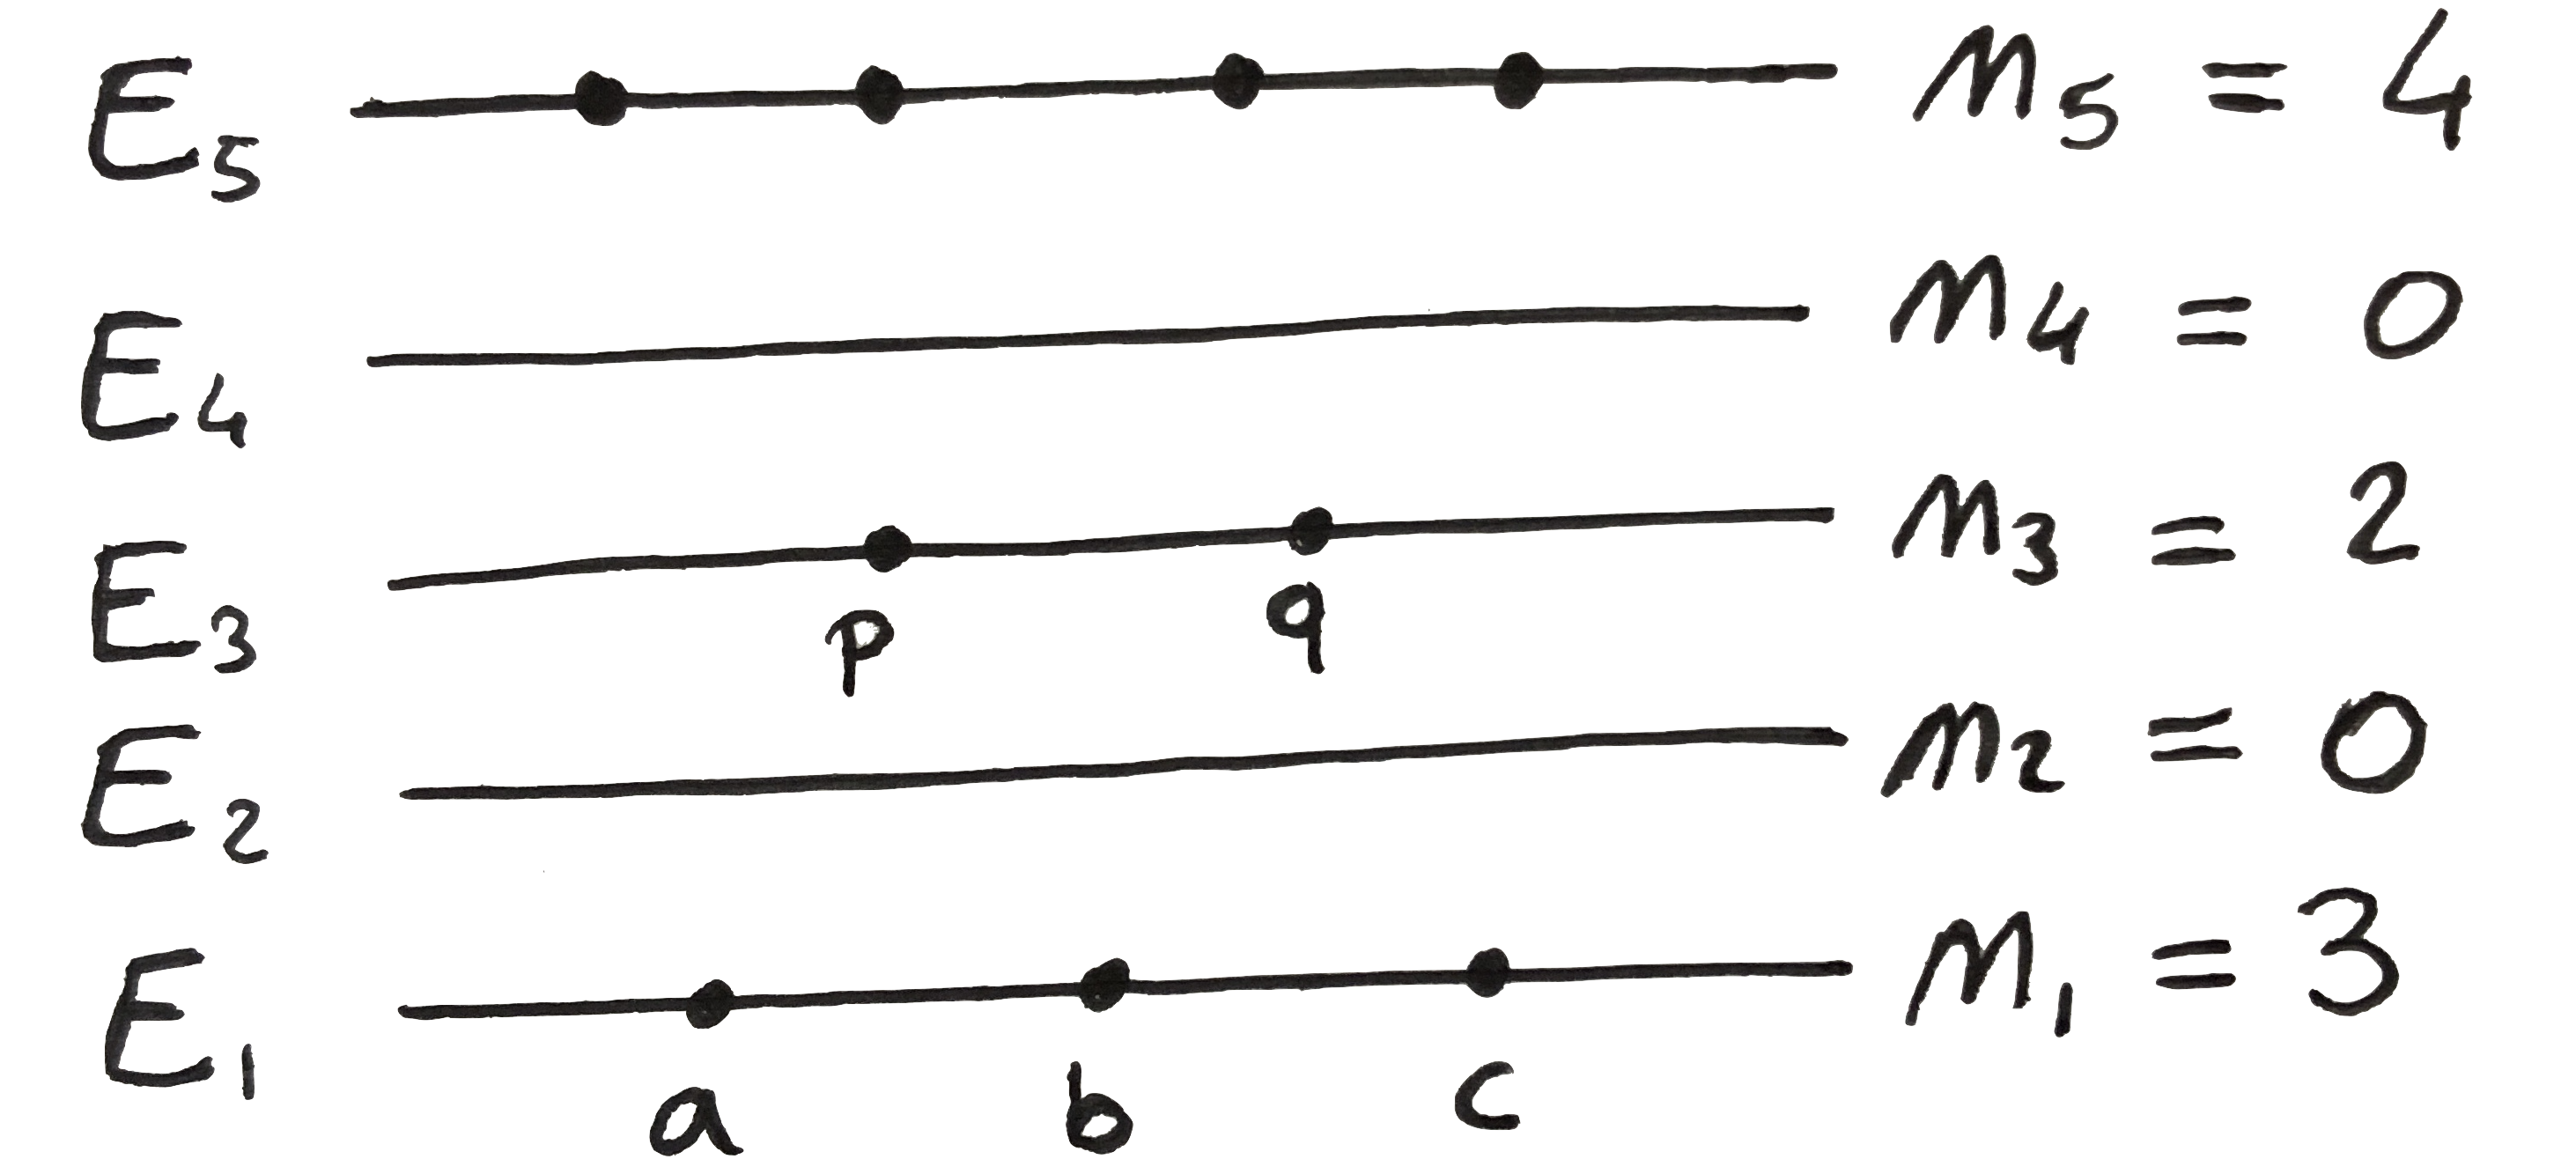
\includegraphics[scale=0.08]{/livelli_energetici_maxwellboltzmann}
\caption{Esempio e rappresentazione della distriubuzione di Maxwell-Boltzmann}
\end{figure}

Questa è una possibile partizione.
Si assume che tutti gli stati di energia abbiano la stessa probabilità di essere occupati.
La probabilità di avere una partizione sarà proporzionale al numero di modi diversi con cui la si può scrivere.
Cioè se pongo fissi gli $n_i$, passo anche le altre particelle in ogni stato (esempio: $p$ al posto di $a$). 
Considero dunque il numero di modi diversi con cui si può costruire la partizione.
Ho $N$ scelte per la prima particella da mettere nel livello corrispondente a $E_1$, $(N-1)$ per la seconda e $(N-2)$ per la terza.
Dunque si ha che il numero di modi con cui si può posizionare particelle nel primo livello energetico è $\frac{N!}{(N-3)!}$.
Tuttavia potrò cambiare l'ordine e avere quindi $abc$, $bca$, $cab$, $bac$, $acb$, $cba$ cioè posso ordinare le particelle in $6 = 3!$ modi diversi,
ma che corrispondono alla stessa partizione in quanto in uno stesso stato le particelle non sono distinguibili.
Si ottiene quindi: $ \frac{N!}{3! (N-3)!} = P_1 $;
$$ \mbox{ che in generale diventa: } P_1 = \frac{N!}{n_1! (N-n_1)!} $$

Passando al secondo livello energetico occorrerà sostituire $N$ con $(N-1)$, da cui si avrà che:
$$ P_2 = \frac{(N-n_1)!}{n_2! ( N - n_1 - n_2)!} $$
E così il terzo:
$$ P_3 = \frac{(N-n_1 - n_2)!}{n_3! ( N - n_1 - n_2 - n_3)!} $$

Ed in generale si ha il numero di modi possibili per ottenere la partizione:

$$ W =  \prod_s P_s = \frac{N!}{n_1! n_2! n_3! ... }  $$

Tuttavia ogni stato dell'energia può essere degenere, ovvero:
può succedere che esista un numero diverso di stato $g_i$ aventi la stessa energia.

Dunque $P_1 = \frac{N! g_1^{n_1}}{n_1! (N - n_1)!}$

$$ \mbox{in generale: } W =  \prod_s P_s = N! \prod_s \frac{g_s^{n_s}}{n_s!} $$

La distribuzione più probabile è quella che massimizza $W$, tenendo conto di alcuni vincoli.

$$ \mbox{1) } \sum_s n_s = N  $$
$$ \mbox{2) } \sum_s n_s E_s = U_{tot}  $$

Considero $\ln(W)$ per passare da produttoria a sommatoria:

$$ \delta \bigl( \ln(W)  \bigr) = \sum_s \frac{\partial \ln(W) }{ \partial n_s } \delta n_s  $$

$$ \delta N = \sum_s \delta n_s = 0 = \delta U = \sum_s E_s \delta n_s $$

$$ \delta \bigl( \ln(W)  \bigr) - \alpha \sum_s \delta n_s - \beta \sum_s E_s \delta n_s = 0 $$

con $\alpha$, $\beta$ moltiplicatori di Lagrange

$$ \ln(W) = \ln N! + \sum_s \bigl[  n_s \ln(g_s) - \ln(n_s!)  \bigr] $$

Applicando l'approssimazione di Stirling $ \bigl[  \ln(n!) \to n \ln(n) - n  \bigr] \iff n \to \infty $

$$ \ln(W) = \ln(N!) + \sum_s \bigl[  n_s \ln(g_s) - n_s \ln(n_s) + n_s \bigr] $$

$$ \delta \bigl( \ln(W) \bigr) = \sum_s \bigl[  \ln(g_s) - \ln(n_s) + 1 - 1 \bigr] \delta n_s $$

$$  \sum_s \bigl[  \ln(g_s) - \ln(n_s) + 1 - 1 \bigr] \delta n_s  - \alpha \sum_s \delta n_s - \beta \sum_s E_s \delta n_s = 0 $$

$$ \sum_s \bigl[  \ln(g_s) - \ln(n_s) - \alpha - \beta E_s \bigr] \delta n_s = 0  $$

$$  \ln \Bigl(  \frac{g_s}{n_s} \Bigr) = \alpha + \beta E_s  \Rightarrow \ln  \Bigl(  \frac{n_s}{g_s} \Bigr)  = - \alpha - \beta E_s  $$

si ottiene così la \textbf{Legge di Distribuzione di Maxwell-Boltzmann:}

$$ n_s = g_s e^{ - \alpha - \beta E_s } $$

Tale formula esprime i valori di $n_s$ che massimizzano $W$.

$$ N = \sum_s n_s = \sum_s g_s e^{- \alpha - \beta E_s} \Rightarrow e^{-\alpha} = \frac{N}{\sum_s g_s e^{ - \beta E_s }} = \frac{N}{Z} $$
$$\mbox{dove } Z = \sum_s g_s e^{ - \beta E_s } $$

\begin{equation}
\begin{cases}
	e^{- \alpha = \frac{N}{Z}} \\
	n_s = \frac{N}{Z} g_s e^{ - \beta E_s }
\end{cases}
\end{equation}



\item  $\Bigr)$
\emph{\textbf{Statistica di Bose-Einstein}}: statistica dei \textit{bosoni}, lavorando nella meccanica quantistica non è possibile distinguere le particelle.

Consideriamo un livello di energia $s$ che sia degenere in $g_s$ stati.

\begin{figure}[h]
\centering
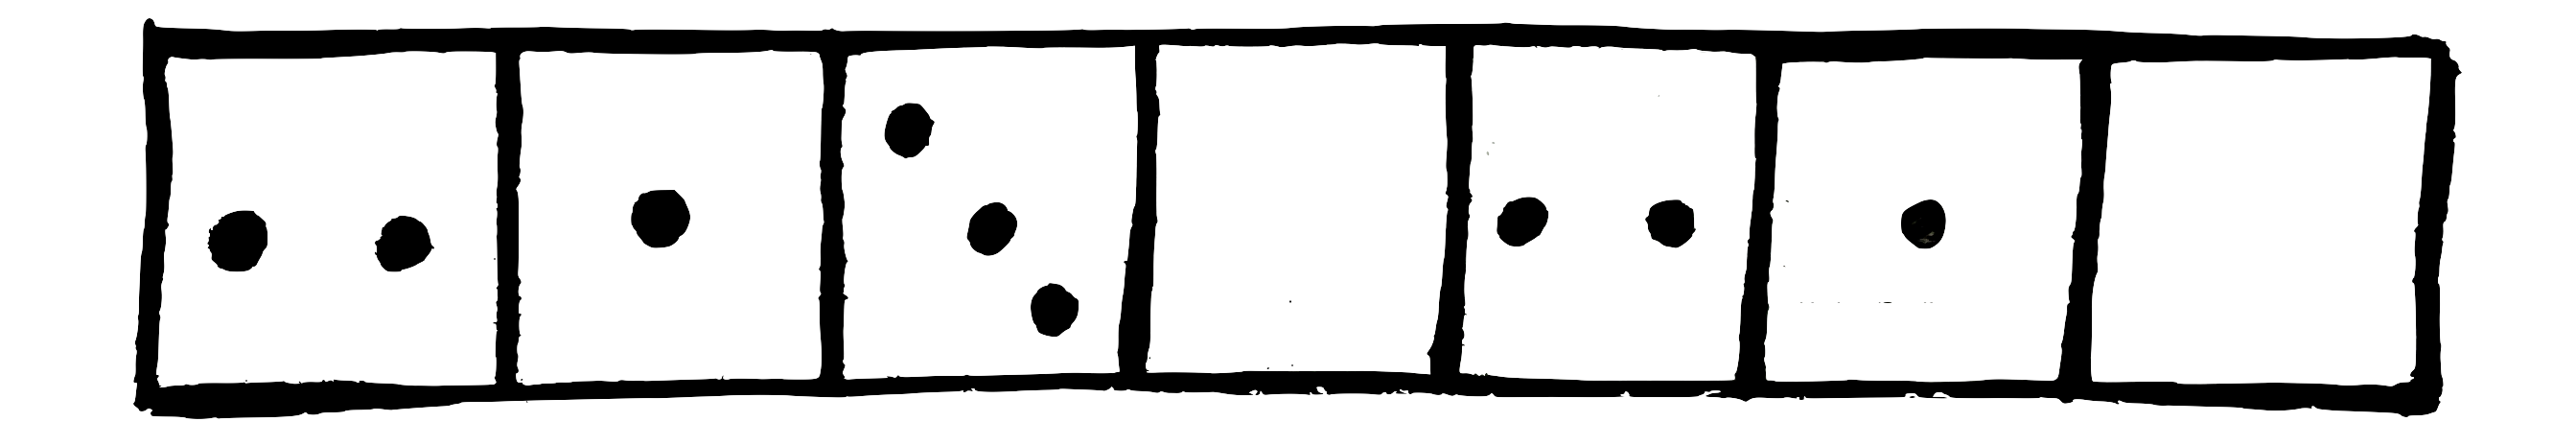
\includegraphics[scale=0.08]{/esempioStatistica_BoseEinstein}
\caption{Esempio e rappresentazione della distriubuzione di Bose-Einstein}
\end{figure}

In questo esempio ci sono 7 stati e quindi 6 linee di divisione.

Il numero totale di particelle $(n_s)$ più il numero di linee di divisione $(g_s - 1)$ è quindi $(n_s + g_s - 1)$.
Posso ottenere un altro modo per la stessa partizione permutando particelle e linee di divisione:
quindi si ha che il numero di modi $\# modi = ( n_s + g_s - 1 )$, ma alcune permutazioni non generano nuovi modi allora avrò:

$$ \frac{(n_s + g_s - 1)!}{n_s! (g_s -1)! } = P_s   \Rightarrow W = \prod_s \frac{(n_s + g_s -1)! }{ n_s! (g_s - 1)! }$$

$$ \ln(W) = \sum_s \Bigl[  \ln(n_s + g_s - 1)! - \ln(n_s !) - \ln(( g_s - 1 )! )  \Bigr] $$

$$ \delta (\ln W ) = \sum_s \Bigl[  \ln ( n_s + g_s ) - \ln ( n_s )  \Bigr] \delta n_s  $$

$$ \sum_s \Bigl[  \ln ( n_s + g_s ) - \ln ( n_s )  - \alpha - \beta E_s \Bigr] \delta n_s = 0 $$

$$ \ln \Bigl(  \frac{n_s}{n_s + g_s}  \Bigr) = - \alpha - \beta E_s $$

si ottiene così la \textbf{Legge di Distribuzione di Bose-Einstein:}

$$ n_s = \frac{g_s}{ e^{\alpha + \beta E_s} - 1 } $$



\item $\Bigr)$
\emph{\textbf{Statistica di Fermi-Dirac}}: statistica dei \textit{fermioni}.

I fermioni sono soggetti al Principio di Esclusione di Pauli, per cui non è possibile avere più particelle in uno stesso stato quantistico.

Consideriamo $n_s$ stati occupati e quindi $(g_s - n_s) = $ stati non occupati.

$$ P_s = \frac{g_s}{n_s! (g_s - n_s)!}  \Rightarrow W = \prod_s P_s = \prod_s \frac{g_s}{n_s! (g_s - n_s)!} $$

$$ \ln W = \sum_s \Bigl[  \ln (g_s!) - \ln (n_s!) - \ln ((g_s - n_s)!)   \Bigr] $$

$$ \delta (\ln W) = \sum_s  \Bigl[ - \ln (n_s) + \ln ((g_s - n_s))   \Bigr]  \delta n_s $$

$$  \sum_s  \Bigl[  - \ln (n_s) + \ln ((g_s - n_s)) - \alpha - \beta E_s \Bigr]  \delta n_s = 0  $$

$$  \ln \Bigl( \frac{n_s}{g_s - n_s}  \Bigr) = - \alpha - \beta E_s  $$

si ottiene così la \textbf{Legge di Distribuzione di Fermi-Dirac:}

$$ n_s = \frac{g_s}{ e^{\alpha + \beta E_s} + 1 } $$


\end{enumerate}



